\documentclass[11pt]{article}

% ====== Packages ======
\usepackage[T1]{fontenc}
\usepackage[utf8]{inputenc}  % if you use XeLaTeX/LuaLaTeX, remove this and set fonts directly
\usepackage{lmodern}
\usepackage{microtype}
\usepackage[margin=1in]{geometry}
\usepackage{setspace}
\usepackage{xcolor}
\usepackage{graphicx}
\usepackage{subcaption}
\usepackage{booktabs}
\usepackage{siunitx}
\usepackage{amsmath,amssymb}
\usepackage{enumitem}
\usepackage{hyperref}
\usepackage[capitalize,noabbrev]{cleveref}
\usepackage{listings}
\usepackage{caption}

% ====== Listings (code) style ======
\lstdefinestyle{mystyle}{
  basicstyle=\ttfamily\small,
  frame=single,
  breaklines=true,
  columns=fullflexible,
  numbers=left,
  numberstyle=\tiny,
  xleftmargin=1.5em,
  showstringspaces=false
}
\lstset{style=mystyle}

% ====== Hyperref colors ======
\hypersetup{
  colorlinks=true,
  linkcolor=blue!50!black,
  citecolor=blue!50!black,
  urlcolor=blue!50!black
}

% ====== Clever helpers ======
\newcommand{\etal}{\textit{et~al.}}
\newcommand{\ie}{i.e., }
\newcommand{\eg}{e.g., }

% ====== Project knobs (edit here to reflect final runs) ======
\newcommand{\NumRoutersA}{64}         % 4x4x4
\newcommand{\NumRoutersB}{64}         % 8x8 (2D baseline with same count)
\newcommand{\Ruby}{Garnet 3.0}
\newcommand{\SimCycles}{2{,}000{,}0}
\newcommand{\Clk}{2\,GHz}
\newcommand{\LinkW}{128\,bits}
\newcommand{\LinkLat}{1}              % ticks
\newcommand{\RouterLat}{1}            % ticks

\title{\textbf{Toward Practical 3D NoCs: Topology Design, Routing Bias, and Cost--Performance Trade-offs}\\
\large A gem5/\Ruby\ Study of 3D Mesh and Sparse-Vertical Variants}
\author{Your Name \quad Your Collaborator\\[2pt]
\small Institution / Course / Term}
\date{\today}

\begin{document}
\maketitle
\doublespacing
\begin{abstract}
This paper studies \emph{practical} 3D Network-on-Chip (NoC) design under
manufacturing and area constraints. Using \texttt{gem5}/\Ruby\ (Garnet 3.0),
we implement dense 3D Mesh and several sparse-Z variants (pillars, hub, torus
augmented) and evaluate them against a same-router-count 2D Mesh under
uniform traffic. We use the throughput \emph{knee} as our primary metric.

\textbf{Key findings.} (i) With equal link latencies, a $4{\times}4{\times}4$
3D Mesh sustains a $\sim$35\% higher threshold throughput than an $8{\times}8$
2D Mesh. (ii) Enabling an \emph{escape virtual channel} (VC$_0$ for an acyclic
route set) amplifies the 3D advantage to $\ge$50--60\%. (iii) In a
\emph{process-aware} setting that penalizes dense 3D with slow Z links
(Z-latency=4) but allows sparse-Z designs to use faster TSVs (Z=1), Torus3D
offers the largest headroom; Mesh3D\_XYZ approaches Mesh\_XY because
\emph{Z-latency dominates}, whereas 2D is constrained by \emph{area/diameter}.
(iv) A TSV-latency sweep shows a consistent \emph{torus multiplier} of
$\approx$2.2–2.4$\times$ in the knee for Sparse3D vs.\ Sparse3D\_Pillars\_torus
(Z$\in\{1,2,4\}$: $\sim$0.10/0.16/0.22 vs.\ $\sim$0.22/0.38/0.50).

\textbf{Guidance.} When TSV budget is limited, prefer sparse-Z to recover
process margin and invest it in reducing effective Z-latency; if floorplan and
timing allow wrap-around, prioritize torus before micro-topology tweaks; and
use an escape VC to safely harvest 3D path diversity.
\end{abstract}

\section{Introduction}
2D NoCs are mature and easy to implement, but their average distance and
bisection bandwidth ultimately limit throughput. 3D organizations add the
Z dimension to shorten paths and raise bandwidth density, yet dense per-router
TSVs stress yield, thermals, and timing. In practice, designers trade Z
\emph{density} for TSV \emph{quality}, and decide whether wrap-around (torus)
is feasible in area and timing.

This paper takes a \emph{process-aware} view of 3D NoCs. We model TSV quality
via a Z-link latency parameter and explore (i) dense 3D Mesh, (ii) sparse-Z
pillars and hub variants that can plausibly use faster TSVs, and (iii) torus
augmentations. We also evaluate the role of an \emph{escape VC}, which
guarantees deadlock-freedom while letting other VCs exploit 3D path diversity.

\paragraph{Questions.}
(1) How large is the 3D advantage over a same-router-count 2D Mesh under equal
latencies, and how does an escape VC change it? (2) When TSV process penalizes
dense Z but benefits sparse-Z designs, which organization retains more of the
3D benefit? (3) How strong is the torus effect across TSV qualities?


\begin{itemize}[leftmargin=1.2em]
  \item \textbf{Implementations.} Configurable topologies in
        \texttt{configs/topologies}: dense 3D Mesh, Cluster3D\_Hub,
        Sparse3D\_Pillars, SW3D\_Express, Hier3D\_Chiplet, and torus variants,
        with weight-based TABLE routing and explicit ports.
  \item \textbf{Reproducible method.} Injection sweeps on \texttt{gem5}/\Ruby\
        with a knee detector; fairness controls (same VC count/buffers,
        link/router latencies unless stated); and a \emph{process-aware}
        mixed-latency setup.
  \item \textbf{Findings.} Equal-latency baseline: 3D $>$ 2D by $\sim$35\%;
        adding an escape VC raises the 3D gap to $\ge$50–60\%.
        When dense Z is penalized (Z=4) but sparse-Z uses faster TSVs (Z=1),
        torus provides the largest headroom and Mesh3D\_XYZ $\approx$ Mesh\_XY.
        Z-latency sweeps show a stable torus multiplier of
        $\approx$2.2–2.4$\times$ in the knee.
  \item \textbf{Guidance.} If area allows wrap-around, enable torus first; else,
        use sparse-Z to gain TSV process margin and reduce effective Z-latency.
        In either case, keep an escape VC to safely exploit 3D path diversity.
\end{itemize}

\section{Background and Related Work}

\ \ \ \ \textbf{Routing models.} Dimension-order routing (XY/XYZ) is deadlock-free by
construction. TABLE routing assigns per-port weights to bias directions.
Reserving one \emph{escape VC} (VC$_0$) for an acyclic route set guarantees
progress while other VCs exploit adaptivity.

\textbf{TSV economics $\rightarrow$ Z-latency.} Dense per-router TSVs raise
yield and thermal risk; sparse-Z lowers TSV count and often enables better
process/stacking. We proxy TSV quality with a Z-link latency parameter.

\textbf{3D organizations.} Prior work spans dense meshes, pillar/hub sharing,
express/long links, chiplet hierarchies, and torus wrap-arounds. We evaluate
representative instances of these families with consistent router/link settings
and a throughput-knee metric tailored to process-aware comparisons.

\section{Topologies Implemented}
This work adds Python topologies under \texttt{configs/topologies/}. All use \texttt{IntLink}/\texttt{ExtLink} wiring with explicit port names (e.g., \texttt{East}, \texttt{UpGW}, \texttt{EastExp}) and \emph{weights} to guide TABLE routing.

\subsection{3D Mesh (XYZ DOR baseline)}
\label{sec:mesh3d}
We use a standard 3D Mesh (e.g., $4{\times}4{\times}4$) with fully populated Z links and DOR (XYZ) or TABLE routing with $W_X < W_Y < W_Z$.
\begin{itemize}[leftmargin=1em]
  \item \textbf{Goal}: establish the upper-bound efficiency for a given router count.
  \item \textbf{parameters}: link/router latency=1; vc = 4 (default); sim-cycle = 20000; link-width=128; GlobalFrequency=2GHz.
\end{itemize}
\begin{figure}[htbp]
    \centering
    \begin{subfigure}[t]{0.45\linewidth}
        \centering
        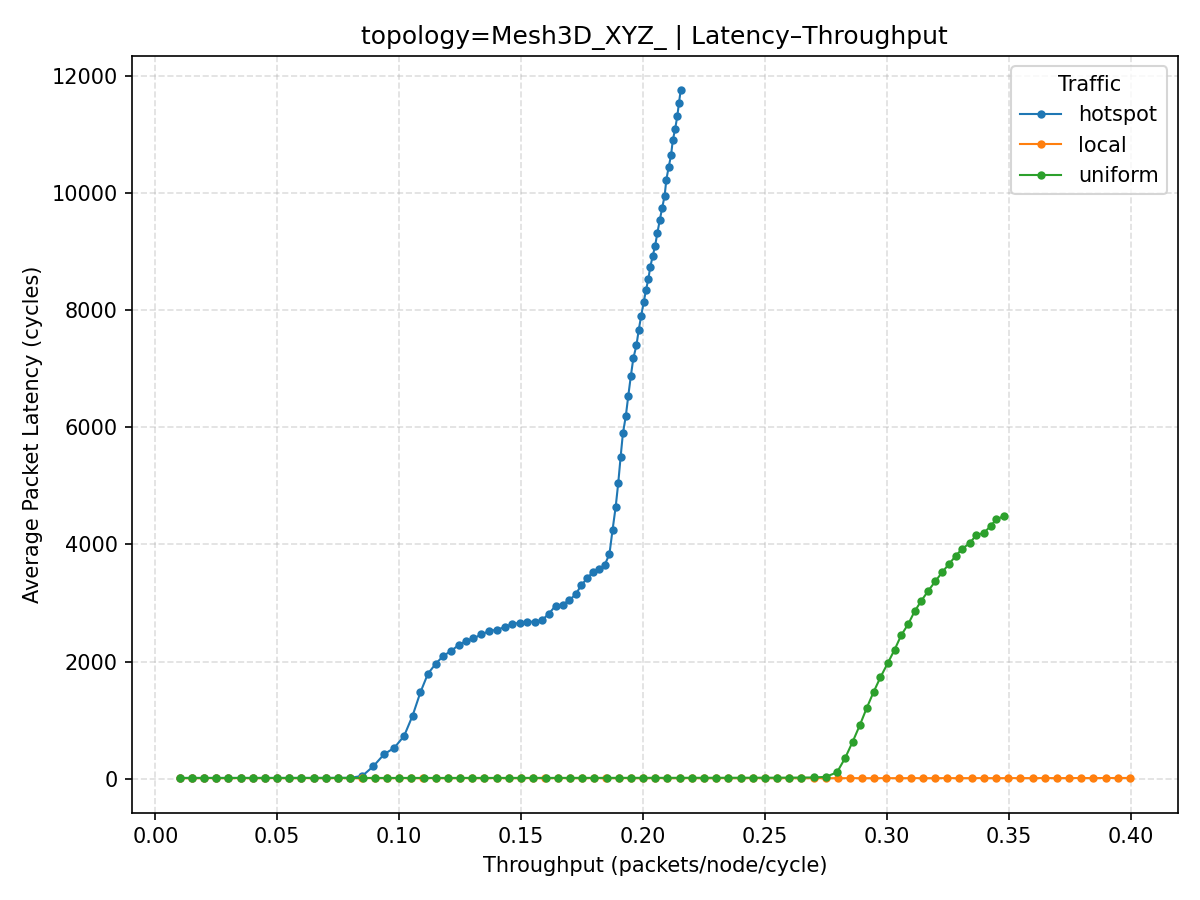
\includegraphics[width=\linewidth]{./figs/Mesh3D-traffic.png}
        \caption{Throughput of the 3D Mesh topology under varying injection rates across different traffic patterns. Uniform traffic achieves the highest sustained throughput, while hotspot traffic saturates earlier due to localized congestion. Local traffic benefits from short paths and maintains high efficiency.}
        \label{fig:mesh3d-throughput}
    \end{subfigure}
    \hfill
    \begin{subfigure}[t]{0.45\linewidth}
        \centering
        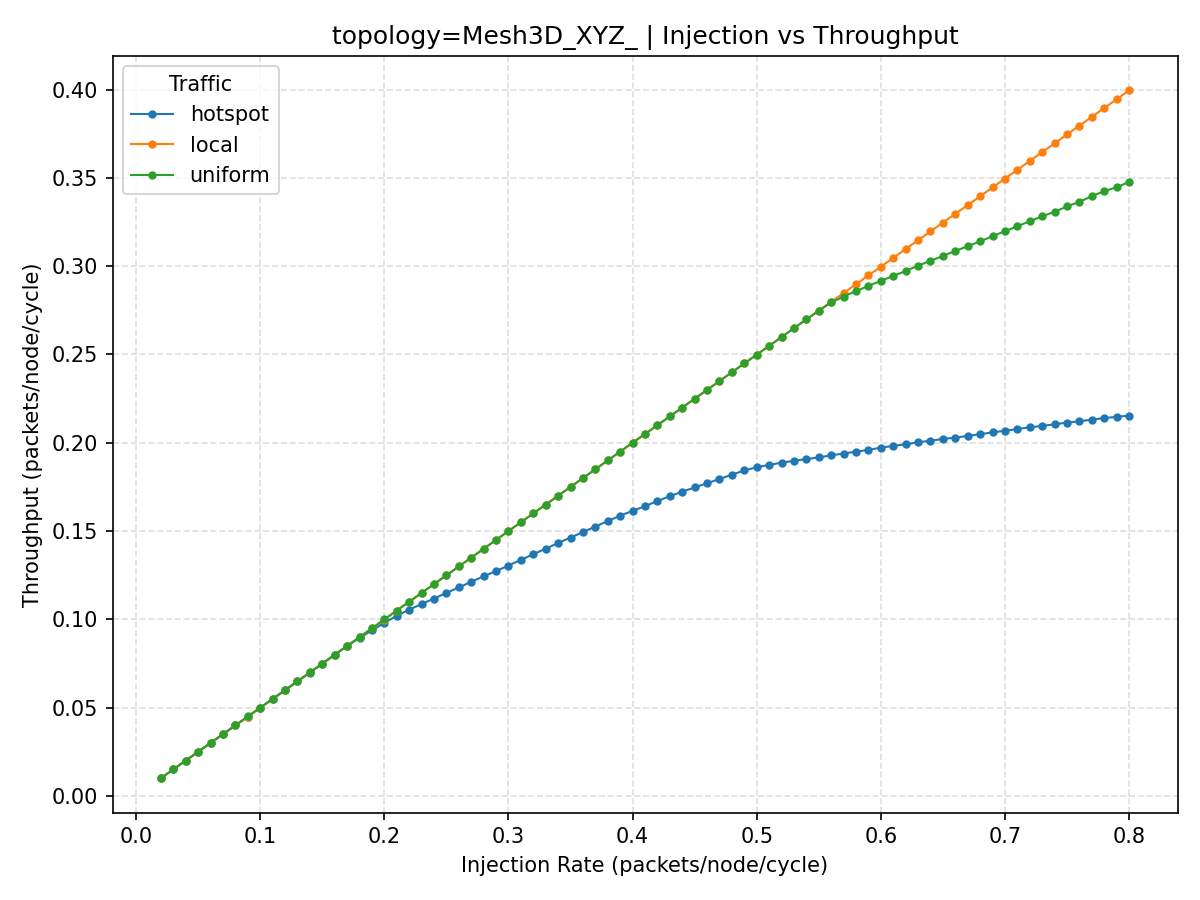
\includegraphics[width=\linewidth]{./figs/Mesh3D-inj_rate-throughput.png}
        \caption{Average packet latency versus throughput for the 3D Mesh network. At low loads, latency remains low; however, as the network approaches saturation, hotspot traffic experiences a sharp rise in latency, while uniform traffic maintains stability up to higher throughput levels.}
        \label{fig:mesh3d-latency-throughput}
    \end{subfigure}
    \caption{Performance evaluation of the 3D Mesh topology under three canonical traffic patterns: (a) throughput vs.\ injection rate, and (b) latency-throughput trade-off. Results demonstrate that although 3D Mesh offers strong baseline performance, its behavior varies significantly with traffic distribution, especially under congestion.}
    \label{fig:mesh3d-performance}
\end{figure}

\subsection{Cluster3D\_Hub}
A $2{\times}2$ submesh per layer shares a central hub; hubs connect vertically. The hub is transit-only (no endpoint injection). We bias routes via weights to funnel local traffic through its hub for Z.
\begin{itemize}[leftmargin=1em]
  \item \textbf{Design knobs}: cluster size (e.g., $2{\times}2{\times}1$, $2{\times}2{\times}2$), vertical speedup, hub router latency reduction.
  \item \textbf{Rationale}: cut TSV count while preserving short detours to vertical resources.
\end{itemize}

\subsection{Sparse3D\_Pillars}
Place vertical pillars every $(P_x, P_y)$ tiles. Only routers aligned to a pillar get Up/Down links. Traffic uses XY detours to the nearest pillar, then moves vertically.
\begin{itemize}[leftmargin=1em]
  \item \textbf{Design knobs}: $P_x,P_y$ spacing, aligned vs.\ staggered patterns (future work).
  \item \textbf{Routing}: TABLE with $W_X<W_Y<W_Z$ and no direct Up/Down from non-pillar routers.
\end{itemize}

\subsection{SW3D\_Express}
Add a budget of long-range \emph{express} links (in-plane or cross-layer) on top of 3D Mesh or sparse-Z base. We use special port names (\texttt{EastExp}, \texttt{UpExp}, \ldots) and assign them the lowest weight ($W_{\text{EXP}}$).
\begin{itemize}[leftmargin=1em]
  \item \textbf{Design knobs}: grid-based placement period $K$ (rule-based); total budget $B$; (optional) randomized placement.
  \item \textbf{Routing}: TABLE prefers express edges first, then normal links.
\end{itemize}

\subsection{Hier3D\_Chiplet}
Partition the die into chiplets (e.g., $4{\times}4{\times}1$ each). Within a chiplet: local mesh. Gateways (1--2 per chiplet) connect to a backbone (2D in-layer and/or vertical). Gateways use \texttt{*GW} ports and higher weights at the backbone to avoid overuse.
\begin{itemize}[leftmargin=1em]
  \item \textbf{Design knobs}: chiplet dimensions, \#gateways, backbone topology (ring/mesh), vertical gateway connectivity.
  \item \textbf{Routing}: TABLE with tiered weights: $W_{\text{intra}} < W_{\text{backbone}} < W_Z$.
\end{itemize}

\begin{table}[t]
  \centering
  \caption{Topology summary and intended routing bias (lower weight is preferred). Edit with your final parameters.}
  \label{tab:topo-summary}
  \begin{tabular}{lcccc}
    \toprule
    \textbf{Topology} & \textbf{Z budget} & \textbf{Extra links} & \textbf{Routing mode} & \textbf{Weights (X/Y/Z/extra)} \\
    \midrule
    3D Mesh         & dense & none      & TABLE or XYZ DOR & 1/2/3/-- \\
    Cluster3D\_Hub  & sparse hubs & hub vertical & TABLE & 1/2/3/-- (hub Z sped-up) \\
    Sparse3D\_Pillars & pillars $(P_x,P_y)$ & none & TABLE & 1/2/3/-- \\
    SW3D\_Express   & dense/sparse & express & TABLE & 1/2/3/0 (exp) \\
    Hier3D\_Chiplet & per-gateway & backbone & TABLE & 1/2/3/-- (+GW tier) \\
    \bottomrule
  \end{tabular}
\end{table}

\section{Routing and Deadlock Considerations}
We primarily use TABLE-based routing in \Ruby\ with weights to induce preferences:
\begin{itemize}[leftmargin=1em]
  \item \textbf{Strict ordering}: Distinct weights per dimension/tier maintain a partial order and avoid cycles typical in oblivious shortest-path selection.
  \item \textbf{Express edges}: assign the smallest weight (e.g., $W{=}0$) to let the router choose them deterministically before normal links.
  \item \textbf{Gateway tiers}: use intermediate weights for backbone/GW hops to avoid accidental oscillations.
\end{itemize}
We validated reachability via \texttt{config.ini} inspections and by eliminating ``No Route exists from this Router'' fatals during warmup runs.

\section{Methodology}
\subsection{Simulator and Network}
We use \texttt{gem5}  with \Ruby\ (Garnet 3.0). Unless noted, system and Ruby clocks are 2GHz. Link width \LinkW, link latency \LinkLat, router latency \RouterLat.



\subsection{Metrics}
We collect average packet/flit latency, average hops, total injected/received packets (to derive accepted rate), and average link utilization. Saturation is indicated by the knee where latency diverges and accepted rate flattens.

\section{Experimental Results}
In following experiments, we use transpose traffic patterns to simulate hotspot traffic, and use neighbor traffic patterns to simulate local traffic, and uniform-random is identical to uniform traffic.
\subsection{3D Mesh vs.\ 2D Mesh (same router count)}
\label{sec:mesh-baseline}

We compare a $4{\times}4{\times}4$ 3D Mesh with an $8{\times}8$ 2D Mesh, both using \NumRoutersA\ routers and identical link/router latencies. The 3D topology is expected to achieve lower average hop counts and higher throughput due to shorter paths and improved bisection bandwidth.

As shown in \cref{fig:mesh-comparison-full}, the 3D Mesh supports significantly higher throughput before saturation under uniform and transpose traffic (up to $\sim$0.35 packets/node/cycle), compared to the 2D Mesh's saturation at $\sim$0.21. Moreover, the 3D design reduces average hop count—especially under uniform traffic—from $\sim$5.3 in 2D to $\sim$3.75 in 3D—by leveraging vertical shortcuts.
\begin{figure}[htbp]
    \centering
    \begin{subfigure}[t]{0.45\linewidth}
        \centering
        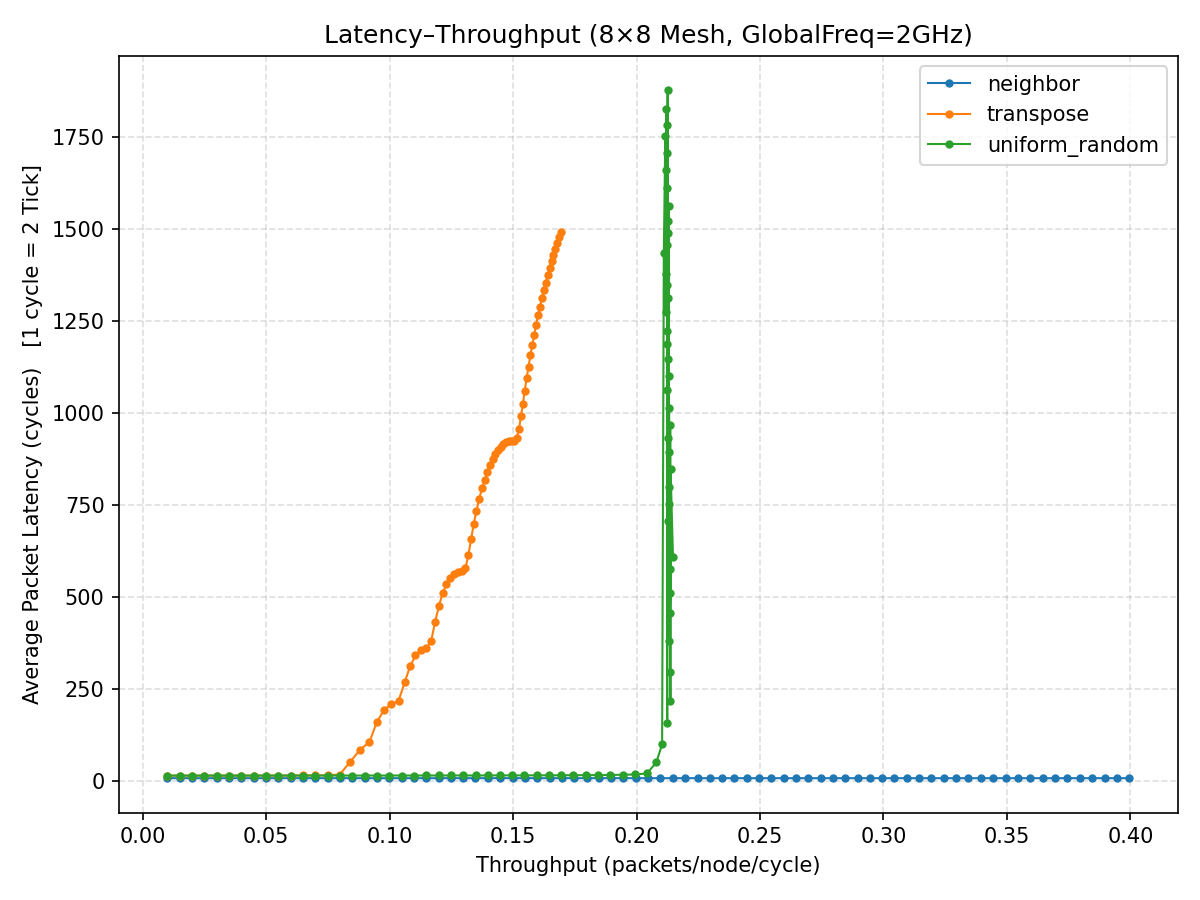
\includegraphics[width=\linewidth]{./figs/Mesh2D-traffic.png}
        \caption{Latency-throughput curve for the $8{\times}8$ 2D Mesh under uniform, transpose, and neighbor traffic patterns. The network saturates at approximately 0.21 packets/node/cycle, with latency diverging sharply under uniform and transpose traffic due to global congestion. Neighbor traffic remains stable due to short paths.}
        \label{fig:mesh2d-latency-throughput}
    \end{subfigure}
    \hfill
    \begin{subfigure}[t]{0.45\linewidth}
        \centering
        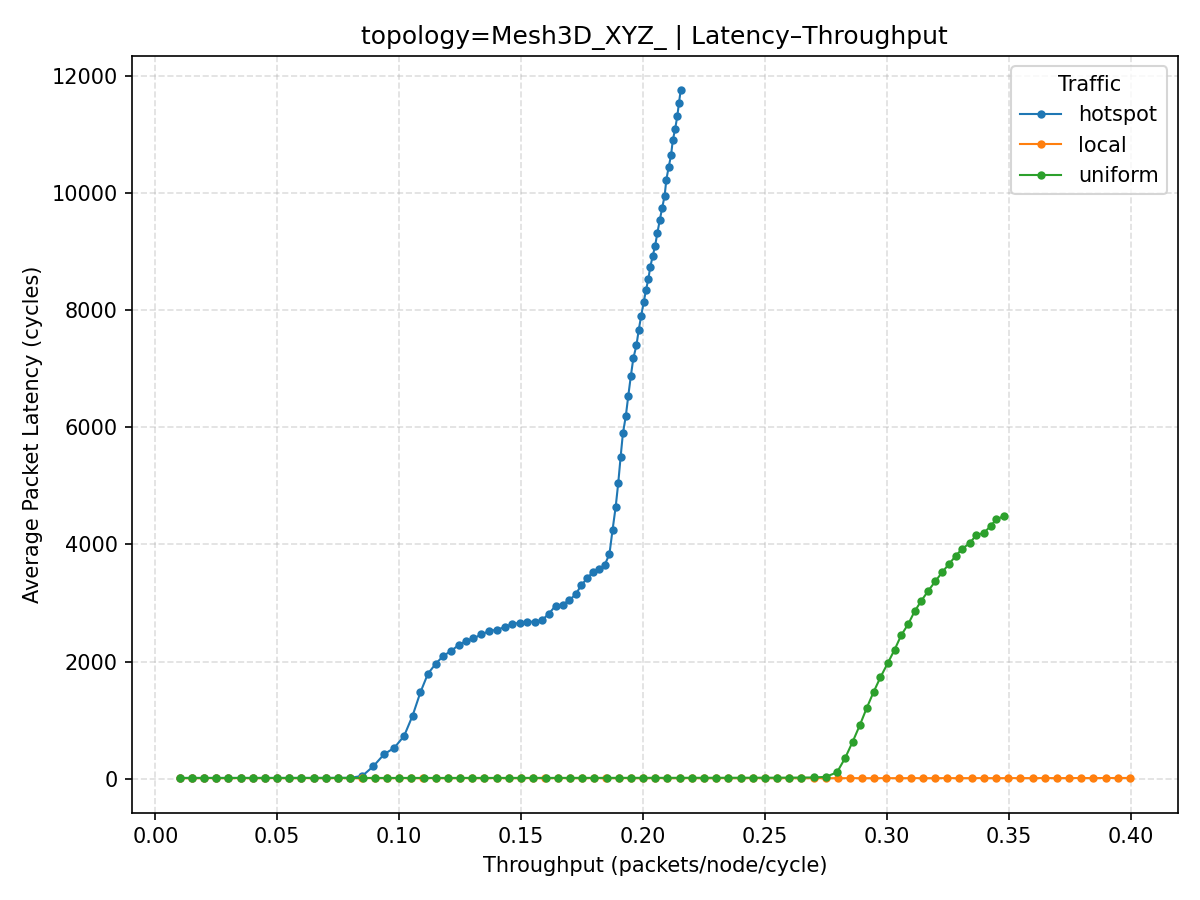
\includegraphics[width=\linewidth]{./figs/Mesh3D-traffic.png}
        \caption{Latency-throughput curve for the $4{\times}4{\times}4$ 3D Mesh under hotspot, local, and uniform traffic. Despite higher average hop counts in some cases, the 3D topology achieves significantly higher throughput before saturation (up to $\sim$0.35), especially under uniform traffic, thanks to reduced path lengths and better bisection bandwidth.}
        \label{fig:mesh3d-latency-throughput}
    \end{subfigure}
    
    \vspace{1em} % 添加垂直间距
    
    \begin{subfigure}[t]{0.45\linewidth}
        \centering
        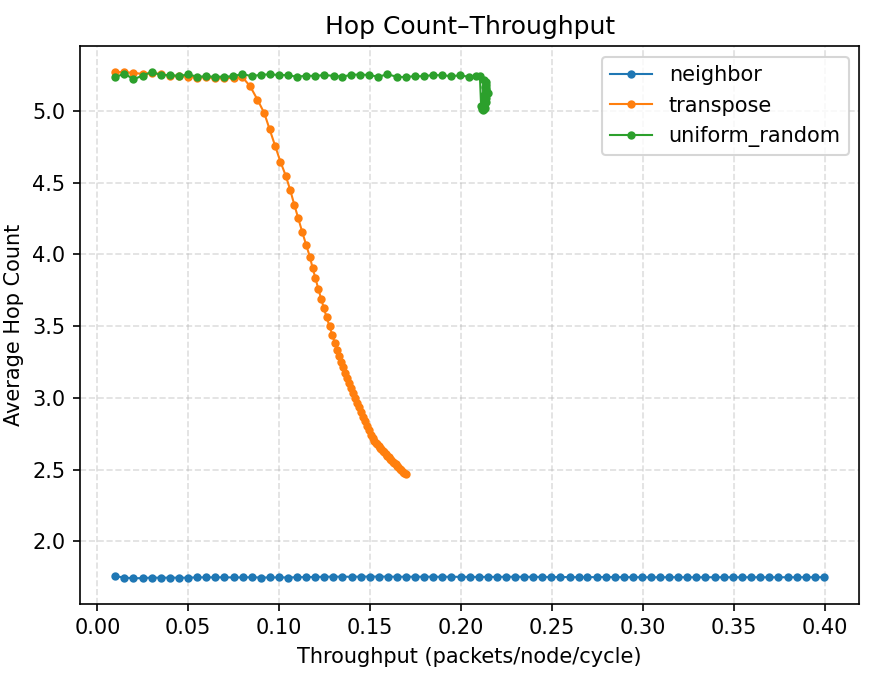
\includegraphics[width=\linewidth]{./figs/Mesh2D_throughput_hops.png}
        \caption{Average hop count versus throughput for the $8{\times}8$ 2D Mesh. Neighbor traffic maintains a constant low hop count ($\sim$1.7) due to short distances. Transpose traffic shows a sharp drop in hop count as injection rate increases, indicating more efficient routing through balanced load distribution. Uniform traffic remains near the theoretical maximum of 5.3 hops across all loads, reflecting long, random paths.}
        \label{fig:mesh2d-hops}
    \end{subfigure}
    \hfill
    \begin{subfigure}[t]{0.45\linewidth}
        \centering
        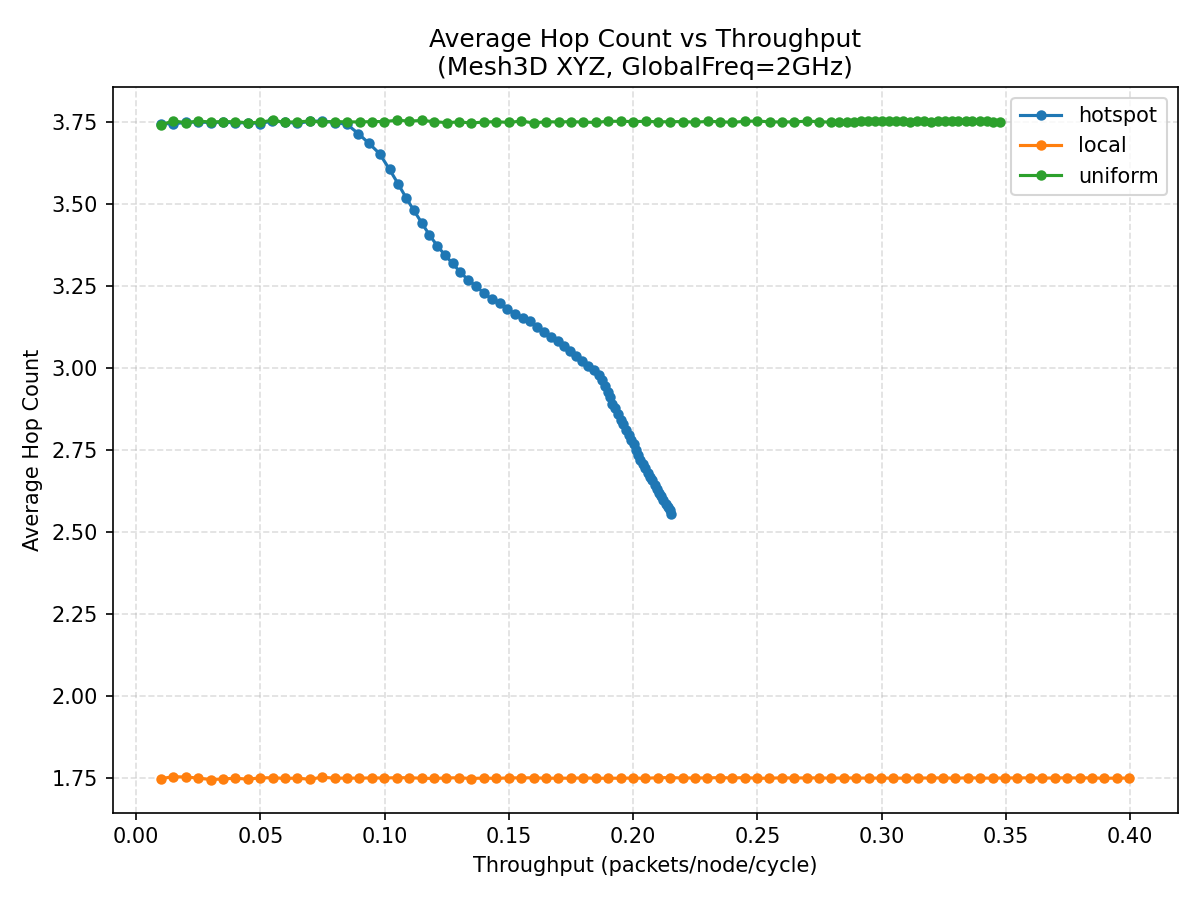
\includegraphics[width=\linewidth]{./figs/Mesh3D_throughput_hops.png}
        \caption{Average hop count versus throughput for the $4{\times}4{\times}4$ 3D Mesh. Local traffic maintains a minimal hop count ($\sim$1.75) throughout, consistent with its short-range nature. Hotspot traffic exhibits a gradual decrease in hop count with increasing load, suggesting adaptive routing or load-balancing effects. Uniform traffic stabilizes at $\sim$3.75 hops, which is significantly lower than the 2D baseline, demonstrating the benefit of Z-dimension shortcuts in reducing average path length.}
        \label{fig:mesh3d-hops}
    \end{subfigure}
    
    \caption{Comparison of performance metrics between 2D Mesh ($8{\times}8$) and 3D Mesh ($4{\times}4{\times}4$) with identical router count (\NumRoutersA). Top row: latency-throughput curves show that the 3D Mesh supports higher throughput and earlier saturation under global workloads. Bottom row: hop count trends reveal that the 3D Mesh reduces average path length, especially under uniform traffic, by leveraging vertical links for shorter routes.}
    \label{fig:mesh-comparison-full}
\end{figure}

\subsection{Effect of Escape VC on 3D vs. 2D}
\label{subsec:escape-vc}
We repeat the uniform-random sweep while enabling an \emph{escape virtual channel} (VC$_0$) reserved for a strictly ordered, deadlock-free route set (e.g., DOR). The remaining VCs use the standard (normal/adaptive) policy. \textbf{All other parameters are kept identical} across 2D and 3D (\texttt{vcs-per-vnet}=4 with one reserved for escape, identical buffers, link/router latencies, clocks, and traffic).


Empirically, the 2D Mesh exhibits a clear knee (threshold throughput) around $\sim$0.21 pkts/node/cycle, whereas the 3D Mesh shows no visible knee up to our maximum offered load of 0.7, achieving accepted throughput $\geq$0.35 in the sweep. Using the \emph{threshold throughput} metric, the relative advantage of 3D increases from about 35\% (without escape VC) to \textbf{$\geq$50--60\%} with escape VC (e.g., $0.35/0.21\approx1.67\times$).


\begin{figure}[htbp]
  \centering
  \begin{subfigure}[t]{0.48\linewidth}
    \centering
    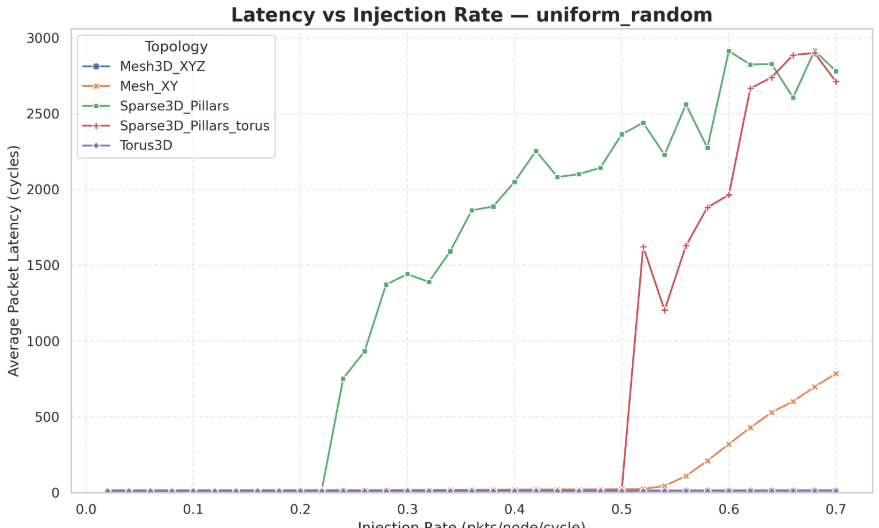
\includegraphics[width=\linewidth]{./figs/escape_lat_vs_inj.png}% TODO: replace with your actual filename
    \caption{Latency vs. injection under uniform-random with escape VC.}
  \end{subfigure}\hfill
  \begin{subfigure}[t]{0.48\linewidth}
    \centering
    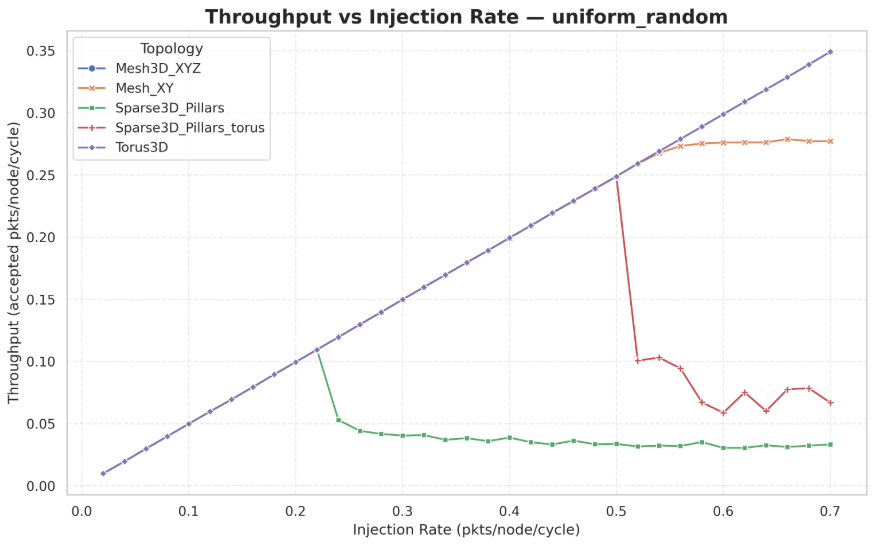
\includegraphics[width=\linewidth]{./figs/escape_thr_vs_inj.png}% TODO: replace with your actual filename
    \caption{Accepted throughput vs. injection under uniform-random with escape VC.}
  \end{subfigure}
  \caption{Escape VC (VC$_0$) amplifies the 3D advantage: 2D shows a knee near $\sim$0.21, while 3D shows no knee up to $\geq$0.35 within our sweep range.}
  \label{fig:escape-vc-results}
\end{figure}


\paragraph{Intuition.} The escape VC guarantees progress, allowing the other VCs to exploit additional turn freedom and transient path diversity. In 3D, the Z dimension supplies more minimal and near-minimal alternatives, so adaptive VCs more effectively relieve head-of-line blocking and allocator contention than in 2D.


\paragraph{Fairness and limits.} Both 2D and 3D reserve exactly one escape VC; buffer sizes and VC counts per input port are identical. Our current sweep upper bound is 0.7 offered load; future work will extend the range to locate the 3D knee more precisely.

\subsubsection{TSV-Latency Sensitivity: Sparse3D vs.\ Sparse3D\_Pillars\_torus}
\label{subsec:z-latency-sweep}

To quantify manufacturing choices, we sweep TSV settings with Z-latency $\in \{1,2,4\}$ for two families:
\emph{Sparse3D\_Pillars} and \emph{Sparse3D\_Pillars\_torus}. The measured
\emph{throughput knees} under uniform traffic are:

\begin{center}
\begin{tabular}{lccc}
\toprule
\textbf{Topology} & \textbf{Z=1} & \textbf{Z=2} & \textbf{Z=4} \\
\midrule
Sparse3D\_Pillars & $\sim$0.10 & $\sim$0.16 & $\sim$0.22 \\
Sparse3D\_Pillars\_torus & $\sim$0.22 & $\sim$0.38 & $\sim$0.50 \\
\bottomrule
\end{tabular}
\end{center}

\begin{figure}[htbp]
  \centering
  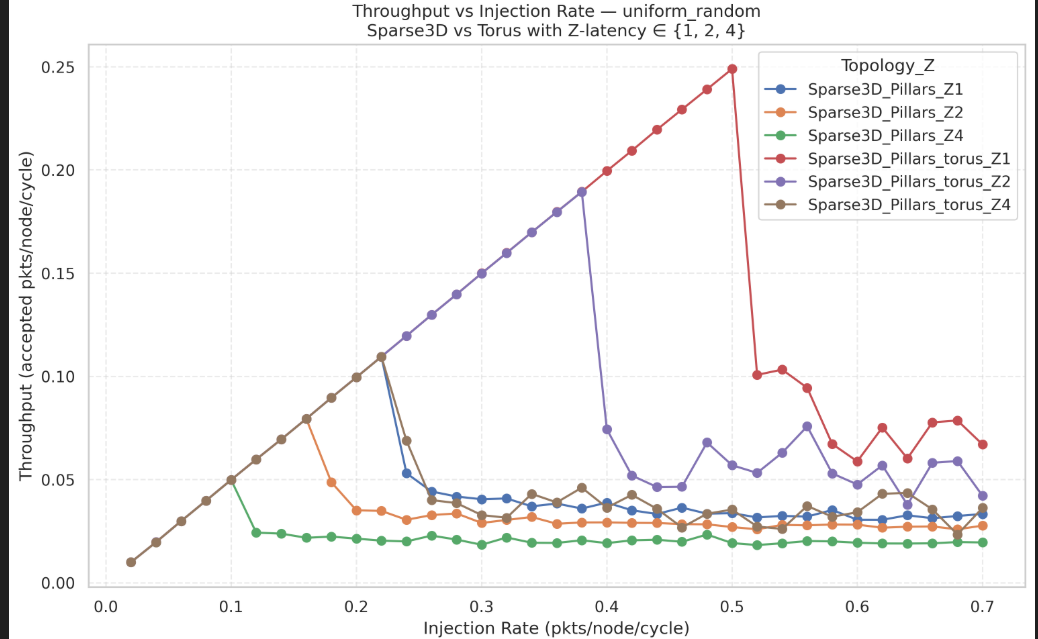
\includegraphics[width=.92\linewidth]{./figs/tsv_latency_sweep_sparse_torus.png}
  \caption{Z-latency sensitivity for Sparse3D vs.\ Sparse3D\_Pillars\_torus under uniform traffic.
  The torus-augmented design consistently pushes the knee higher (about $2.2\!\times$--$2.4\!\times$
  across the three Z settings in our runs).}
  \label{fig:z-latency-sweep}
\end{figure}

\noindent\textbf{Design takeaways.}
\begin{itemize}[leftmargin=1.2em]
  \item \textbf{Torus multiplier.} For the same Z setting, adding torus roughly doubles the knee
        (e.g., $0.22/0.10\!\approx\!2.2$, $0.38/0.16\!\approx\!2.4$, $0.50/0.22\!\approx\!2.3$).
  \item \textbf{Process-first budget use.} If TSV process can be improved for a \emph{sparse} Z budget,
        prioritizing lower effective Z-latency yields a larger payoff than micro-level tweaks on a non-torus grid.
  \item \textbf{Where to spend area.} If floorplan permits wrap-around, torus offers the highest headroom per TSV;
        otherwise, investing TSV quality on a sparse grid still moves the knee materially.
\end{itemize}

\subsection{Process-Aware Case Study: Mixed Z-Link Latency}
\label{subsec:process-aware-mixed-z}

\textbf{Setup.} To emulate realistic manufacturing trade-offs, we keep XY link latency at~1
for all topologies. We penalize the dense 3D mesh by setting its Z links to latency~4
(to reflect TSV difficulty when every router has a TSV), while \emph{sparser-Z} topologies
use Z-latency~=~1 (better TSV process made possible by lower TSV density).

\begin{figure}[htbp]
  \centering
  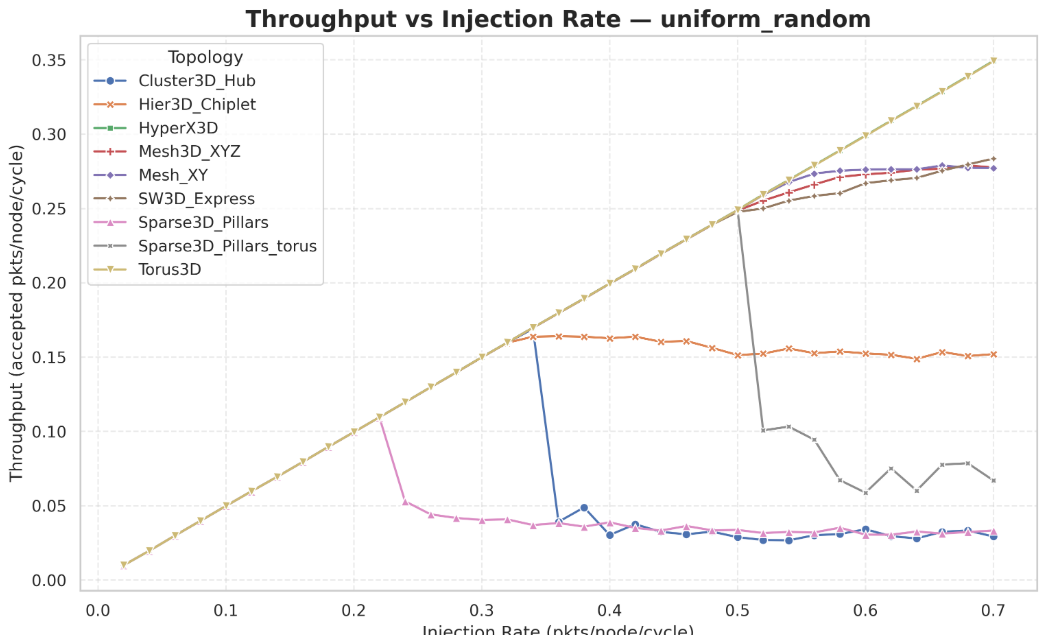
\includegraphics[width=.92\linewidth]{./figs/overview_mixed_zlatency.png}
  \caption{Process-aware comparison under uniform traffic:
  dense 3D mesh uses Z-latency~4; all other sparse-Z designs use Z-latency~1.
  Torus3D shows the largest headroom; Mesh\_XY and Mesh3D\_XYZ become close because
  the latter is bottlenecked by slow Z.}
  \label{fig:process-aware-overview}
\end{figure}

\noindent\textbf{Observations.}
\begin{itemize}[leftmargin=1.2em]
  \item \textbf{Torus impact is substantial.} Torus3D continues scaling to the highest accepted rate
        (cf.\ Fig.~\ref{fig:process-aware-overview}); whether such wrapping can be realized within the
        floorplan and timing is a first-order implementation question.
  \item \textbf{Mesh3D\_XYZ $\approx$ Mesh\_XY under slow Z.} This contrasts with our equal-latency baseline
        where 3D $>$ 2D. Here the 3D advantage is dominated by TSV process (Z-latency), whereas 2D is constrained
        by \emph{area/diameter}. \textit{Process vs.\ area} is therefore a central chip-production trade-off.
  \item \textbf{Generalization to other 3D variants.} Topology evolution alone yields limited gains if the Z process
        is poor; with improved TSV (enabled by sparsity), benefits reappear. Hence, \emph{manufacturing and
        floorplanning constraints often dominate over micro-topology tweaks}.
\end{itemize}


\section{Discussion}
\subsection{Manufacturing-driven guidance.}
Our process-aware study (Secs.~\ref{subsec:process-aware-mixed-z}, \ref{subsec:z-latency-sweep})
shows that (i) Z-latency (TSV quality) can erase or amplify the theoretical 3D gain;
(ii) torus raises the throughput knee by about $2.2$--$2.4\times$ across Z settings in our runs;
(iii) when TSV density is reduced (sparse-Z), the saved process margin can be reinvested to
achieve lower Z-latency and reclaim most of the 3D advantage. In short: \emph{process \& area
choices dominate topology micro-variants}—optimize TSV quality or enable torus first, then tune the grid.


\subsection{Routing Simplicity vs.\ Performance}
TABLE routing with weights gives strong baselines without custom algorithms; we note when custom adaptive schemes might help (left as future work).

\subsection{Limitations}

\section{Conclusion}

\appendix

\section{Topology Implementation Details}
We place our Python files in \texttt{configs/topologies/}: 
\begin{itemize}[leftmargin=1em]
  \item \texttt{Mesh3D\_XYZ\_.py}: 3D Mesh baseline (XYZ DOR or TABLE).
  \item \texttt{Cluster3D\_Hub.py}: cluster hub + vertical hub links (with configurable hub speedup).
  \item \texttt{Sparse3D\_Pillars.py}: pillar spacing $(P_x,P_y)$; optional staggered layout (future).
  \item \texttt{SW3D\_Express.py}: rule-based express placement (period $K$) with $W_{\text{EXP}}{=}0$.
  \item \texttt{Hier3D\_Chiplet.py}: chiplet size, \#gateways, backbone wiring.
\end{itemize}
We followed gem5’s \texttt{Mesh\_XY} style: create routers, wire \texttt{ExtLink}s to NIs, then build \texttt{IntLink}s with port names and weights.

\section{Command Lines and Sweeps}
\subsection*{Single Run Example}
\begin{lstlisting}[language=bash]
./build/NULL/gem5.opt configs/example/garnet_synth_traffic.py \
  --network=garnet --topology=Sparse3D_Pillars \
  --num-cpus=64 --num-dirs=64 --mesh-rows=4 \
  --routing-algorithm=0 \
  --synthetic=uniform_random --injectionrate=0.05 \
  --sim-cycles=2000000 \
  --sys-clock=1GHz --ruby-clock=1GHz \
  --link-width-bits=128 --link-latency=2 --router-latency=2 \
  --mem-type=SimpleMemory --mem-channels=64 --mem-size=8192MB
\end{lstlisting}

\subsection*{Sweep Script (bash)}
\begin{lstlisting}[language=bash]
for r in $(seq 0.01 0.01 0.25); do
  ./build/NULL/gem5.opt \
    -d runs/pillars_uniform_r${r} \
    configs/example/garnet_synth_traffic.py \
    --network=garnet --topology=Sparse3D_Pillars \
    --num-cpus=64 --num-dirs=64 --mesh-rows=4 \
    --routing-algorithm=0 \
    --synthetic=uniform_random --injectionrate=${r} \
    --sim-cycles=2000000 \
    --sys-clock=1GHz --ruby-clock=1GHz \
    --link-width-bits=128 --link-latency=2 --router-latency=2 \
    --mem-type=SimpleMemory --mem-channels=64 --mem-size=8192MB
done
\end{lstlisting}

\section{Data Collection and Plotting}
\label{sec:repro}
\paragraph{Collect CSV.}
\begin{lstlisting}[language=bash]
./collect.sh runs results/pillars_uniform.csv
\end{lstlisting}

\paragraph{Plot curves.}
\begin{lstlisting}[language=bash]
python3 plot_metrics.py \
  --out results/plots \
  --series "Pillars:results/pillars_uniform.csv" \
  --series "3D Mesh:results/mesh3d_uniform.csv"
\end{lstlisting}

\section{Sanity Checks}
We grep \texttt{config.ini} to confirm topology name, routing mode, \#IntLinks, port names (e.g., \texttt{UpGW}, \texttt{EastExp}) and weight histograms; we ensure every router has outgoing \texttt{IntLink}s.

\section*{References}
\bibliographystyle{abbrv}
\bibliography{references}
\end{document}
